\documentclass[9pt,twocolumn,twoside]{pnas-new}
\usepackage{amsmath}
\usepackage{gensymb}
\usepackage{bm}
\usepackage{physics}
\usepackage{booktabs}
\usepackage{textcomp}
\graphicspath{{figures/}}
% Use the lineno option to display guide line numbers if required.
% Note that the use of elements such as single-column equations
% may affect the guide line number alignment. 

\templatetype{pnasresearcharticle} % Choose template
% {pnasresearcharticle} = Template for a two-column research article
% {pnasmathematics} = Template for a one-column mathematics article
% {pnasinvited} = Template for a PNAS invited submission

\title{Development of a 602 nm Laser for use in Germanium Vacancy Excitation}

% Use letters for affiliations, numbers to show equal authorship (if applicable) and to indicate the corresponding author
%\author[a,c,1]{Author One}
%\author[b,1,2]{Author Two} 
%\author[a]{Author Three}
\author[a,1]{Tristan Shoemaker}
\author[a]{Lilian Childress, Prof.}

\affil[a]{Department of Physics, McGill University, 3600 Rue Universit\'{e}, Montr\'{e}eal, QC, H3A 2T8, Canada}

% Please give the surname of the lead author for the running footer
\leadauthor{Shoemaker} 

% Please add here a significance statement to explain the relevance of your work
%\significancestatement{Authors must submit a 120-word maximum statement about the significance of their 
%research paper written at a level understandable to an undergraduate educated scientist outside their field of %speciality. The primary goal of the Significance Statement is to explain the relevance of the work in broad
%context to a broad readership. The Significance Statement appears in the paper itself and is required for all %research papers.}

%\significancestatement{Quantum Computation offers a potential solution to a large class of problems, whose solutions are unfeasible to calculate using classical computation algorithms. Integer factorization of a product of two large primes, the foundation of public-private key cryptography, is an example of such a problem. The ability to efficiently solve such a problem would have huge ramifications in modern computer security and privacy. }

\significancestatement{Quantum networks for use in quantum computation, information and communication applications require quantum nodes that interface photons with material systems capable of storing and processing quantum information\cite{Kimble2008}. Defect centers in diamond provide a promising solution, with long coherence times and convenient optical addressing. The Nitrogen Vacancy (NV) defect is the most studied and has long spin coherence times. The Germanium Vacancy (GeV) is a recently discovered defect with high coherent emission, and the possibility of long spin coherence at cryogenic temperatures \cite{Sukachev2017}. Resonant excitation of the GeV requires a tunable laser source centered around 602nm, a wavelength inaccessible by diode or gas lasers. Dye lasers can be used but require constant maintenance and degrade over time, making frequency doubling an infrared laser is an attractive option for generating this wavelength.}

% Please include corresponding author, author contribution and author declaration information
%\authorcontributions{Please provide details of author contributions here.}
%\authordeclaration{Please declare any conflict of interest here.}
%\equalauthors{\textsuperscript{1}A.O.(Author One) and A.T. (Author Two) contributed equally to this work (remove if not applicable).}
\correspondingauthor{\textsuperscript{1}To whom correspondence should be addressed. E-mail: tristan.shoemaker@mail.mcgill.ca}

% Keywords are not mandatory, but authors are strongly encouraged to provide them. If provided, please include two to five keywords, separated by the pipe symbol, e.g:
\keywords{Frequency Doubling | Nonlinear Optics | Quasi Phase Matching}  
 
\begin{abstract}
%Please provide an abstract of no more than 250 words in a single paragraph. Abstracts should explain to the general reader the major contributions of the article. References in the abstract must be cited in full within the abstract itself and cited in the text.

Germanium vacancy centers in diamond offer a promising solution to a quantum coherent light-matter interface. Further study of this defect requires a wavelength tunable laser source centered around 602nm. To avoid the use of dye lasers, we frequency double an infrared laser source using periodically poled, waveguide confined potassium titanyl phosphate crystal to fulfill this requirement. This paper explores the development of such a laser source, with an effort to maximize output power and tuning range. The result is 335 \textmu W of fiber-coupled 602.7 nm light, with a mode-hop free tuning range of $\sim$0.05 nm. 

\end{abstract}

\dates{This manuscript was compiled on \today}
%\doi{\url{www.pnas.org/cgi/doi/10.1073/pnas.XXXXXXXXXX}}

\begin{document}
\renewcommand{\arraystretch}{1.2}

% Optional adjustment to line up main text (after abstract) of first page with line numbers, when using both lineno and twocolumn options.
% You should only change this length when you've finalised the article contents.
\verticaladjustment{-2pt}

\maketitle
\thispagestyle{firststyle}
\ifthenelse{\boolean{shortarticle}}{\ifthenelse{\boolean{singlecolumn}}{\abscontentformatted}{\abscontent}}{}

% If your first paragraph (i.e. with the \dropcap) contains a list environment (quote, quotation, theorem, definition, enumerate, itemize...), the line after the list may have some extra indentation. If this is the case, add \parshape=0 to the end of the list environment.

\dropcap{F}requency doubling infrared (IR) light is a powerful method for generating visible wavelengths from widely available and well understood semiconductor IR lasers. This project's aim is to use frequency doubling to create a mW level, stable, and tuneable laser source in an otherwise difficult to access wavelength range around 602 nm. Frequency doubling is achieved through Second Harmonic Generation (SHG), which is a nonlinear optical effect that converts an incident electric field of frequency $\omega$ (the ``pump'' field) to a field of frequency $2\omega$ (the SHG field). 

In linear optics, the relation between the polarization $\tilde{P}$ and the electric field $\tilde{E}$ in the material is the linear relationship
\begin{equation*}
	\tilde{P} = \epsilon_0 \chi^{(1)} \tilde{E}(t),
\end{equation*}
with the ratio between them given by the susceptibility $\chi^{(1)}$, and where $\epsilon_0$ is the permittivity of free space. SHG occurs in materials as the result of a nonlinear polarization response to a strong electric field. Following Boyd \cite{Boyd2008} we can express the polarization $\tilde{P}$ as a power series
\begin{equation*}
	\tilde{P}(t) = \epsilon_0 \left[ \chi^{(1)} \tilde{E}(t) + \chi^{(2)} \tilde{E}^2(t) + ... + \chi^{(n)} \tilde{E}^n(t) \right],
\end{equation*}
where the nonlinear response of the crystal is described by a nonlinear susceptibility $\chi^{(n)}$, with the second harmonic being $\chi^{(2)}$. Using this second order nonlinear susceptibility and moving to the Fourier domain, we can then define the second order nonlinear polarizations $P_1$ and $P_2$ for the incident frequency $\omega$ (subscripted $1$) and generated frequency $2\omega$ (subscripted $2$) waves as
\begin{gather*}
	P_1(z) = 2 \varepsilon_0 \chi^{(2)} E_2 E_1^\ast \\
	P_2(z) = \varepsilon_0 \chi^{(2)} E_1^2.
\end{gather*}
where $E_1$ and $E_2$ are the indecent and generated electric field. By expressing the electric field $E_j$ in terms of a slowly varying amplitude $A_j$
\begin{equation*}
	E_j(z) = A_j(z)e^{i k_j z}
\end{equation*}
where the wavevector $k_j = \omega_j \sqrt{\epsilon^{(1)}( \omega_j )} / c$ and $\epsilon^{(1)}( \omega_j )$ is the material permittivity, we can rewrite the polarizations as
\begin{gather*}
	P_1(z) = 2 \varepsilon_0 \chi^{(2)} A_2 A_1^\ast e^{i(k_2-k_1)z} \\
	P_2(z) = \varepsilon_0 \chi^{(2)} A_1^2 e^{2 i k_1 z}.
\end{gather*}
Plugging these expressions into the driven field equation
$$
	\frac{\partial^2 \tilde{E}_j}{\partial z^2} - \frac{\epsilon^{(1)}(\omega_j)}{c^2}\frac{\partial^2 \tilde{E}_j}{\partial t^2} = \frac{1}{\epsilon_0 c^2}\frac{\partial^2}{\partial t^2}\tilde{P}_j,
$$
and applying the slowly-varying envelope approximation, we can derive two coupled-amplitude equations that describe the pump and generated fields in a material with nonlinear susceptability $\chi^{(2)}$. These are
\begin{equation*} \label{equ:a1dz}
	\frac{d A_1}{dz} \propto \chi^{(2)} A_2 A_1^\ast e^{-i \Delta k z}
\end{equation*}
and
\begin{equation} \label{equ:a2dz}
	\frac{d A_2}{dz} \propto \chi^{(2)} A_1^2 e^{i \Delta k z}
\end{equation}
where
\begin{equation} \label{equ:pmc}
	\Delta k = 2k_1 - k_2.
\end{equation}
Integrating equation \ref{equ:a2dz} while keeping $A_1$ constant gives the generated amplitude in the undepleted pump approximation where we assume that a negligibly small percentage of the pump field is converted. Since the output amplitude $A_2$ is proportional to the square of the input field amplitude $A_1$, increasing the input field density is important to efficient conversion. 

Equation \ref{equ:pmc} defines the wavevector mismatch $\Delta k$. This is an important quantity as the maximum second harmonic field amplitude per length can only be produced when $\Delta k = 0$, known as perfect phase matching. Because of the dispersive index of refraction present in most suitable crystals, perfect phase matching is very difficult to achieve. If $\Delta k \neq 0$, then the generated field amplitude will oscillate as a function of distance, with a period of $4L_{coh} = 4 \pi / \Delta k$, preventing a significant SHG field from building up. Therefore, in order to generate a significant SHG field without perfect phase matching, we use Quasi Phase Matching (QPM). In QPM, the sign of $\chi^{(2)}$ is reversed with period $\Lambda = 2 L_{coh}$ to approximate the ideal phase relationship between the pump and generated fields. QPM allows the generated field to accumulate and increase monotonically with crystal length, despite a non-zero wavevector mismatch \cite{Suhara2003}. These three phase matching conditions are shown in Fig. \ref{fig:pedagog} (b), with the general crystal configuration in Fig. \ref{fig:pedagog} (a).

Additionally, an embedded rectangular waveguide is formed on the surface of the crystal using ion exchange. This waveguide confines the pump field to increase the pump field density, and therefore the generated field amplitude. The waveguide also guides the SHG field. Maximizing the SHG field is then dependant on maximizing the coupling between the incoming IR pump field and the waveguide modes.
	
\begin{figure}
	\centering
	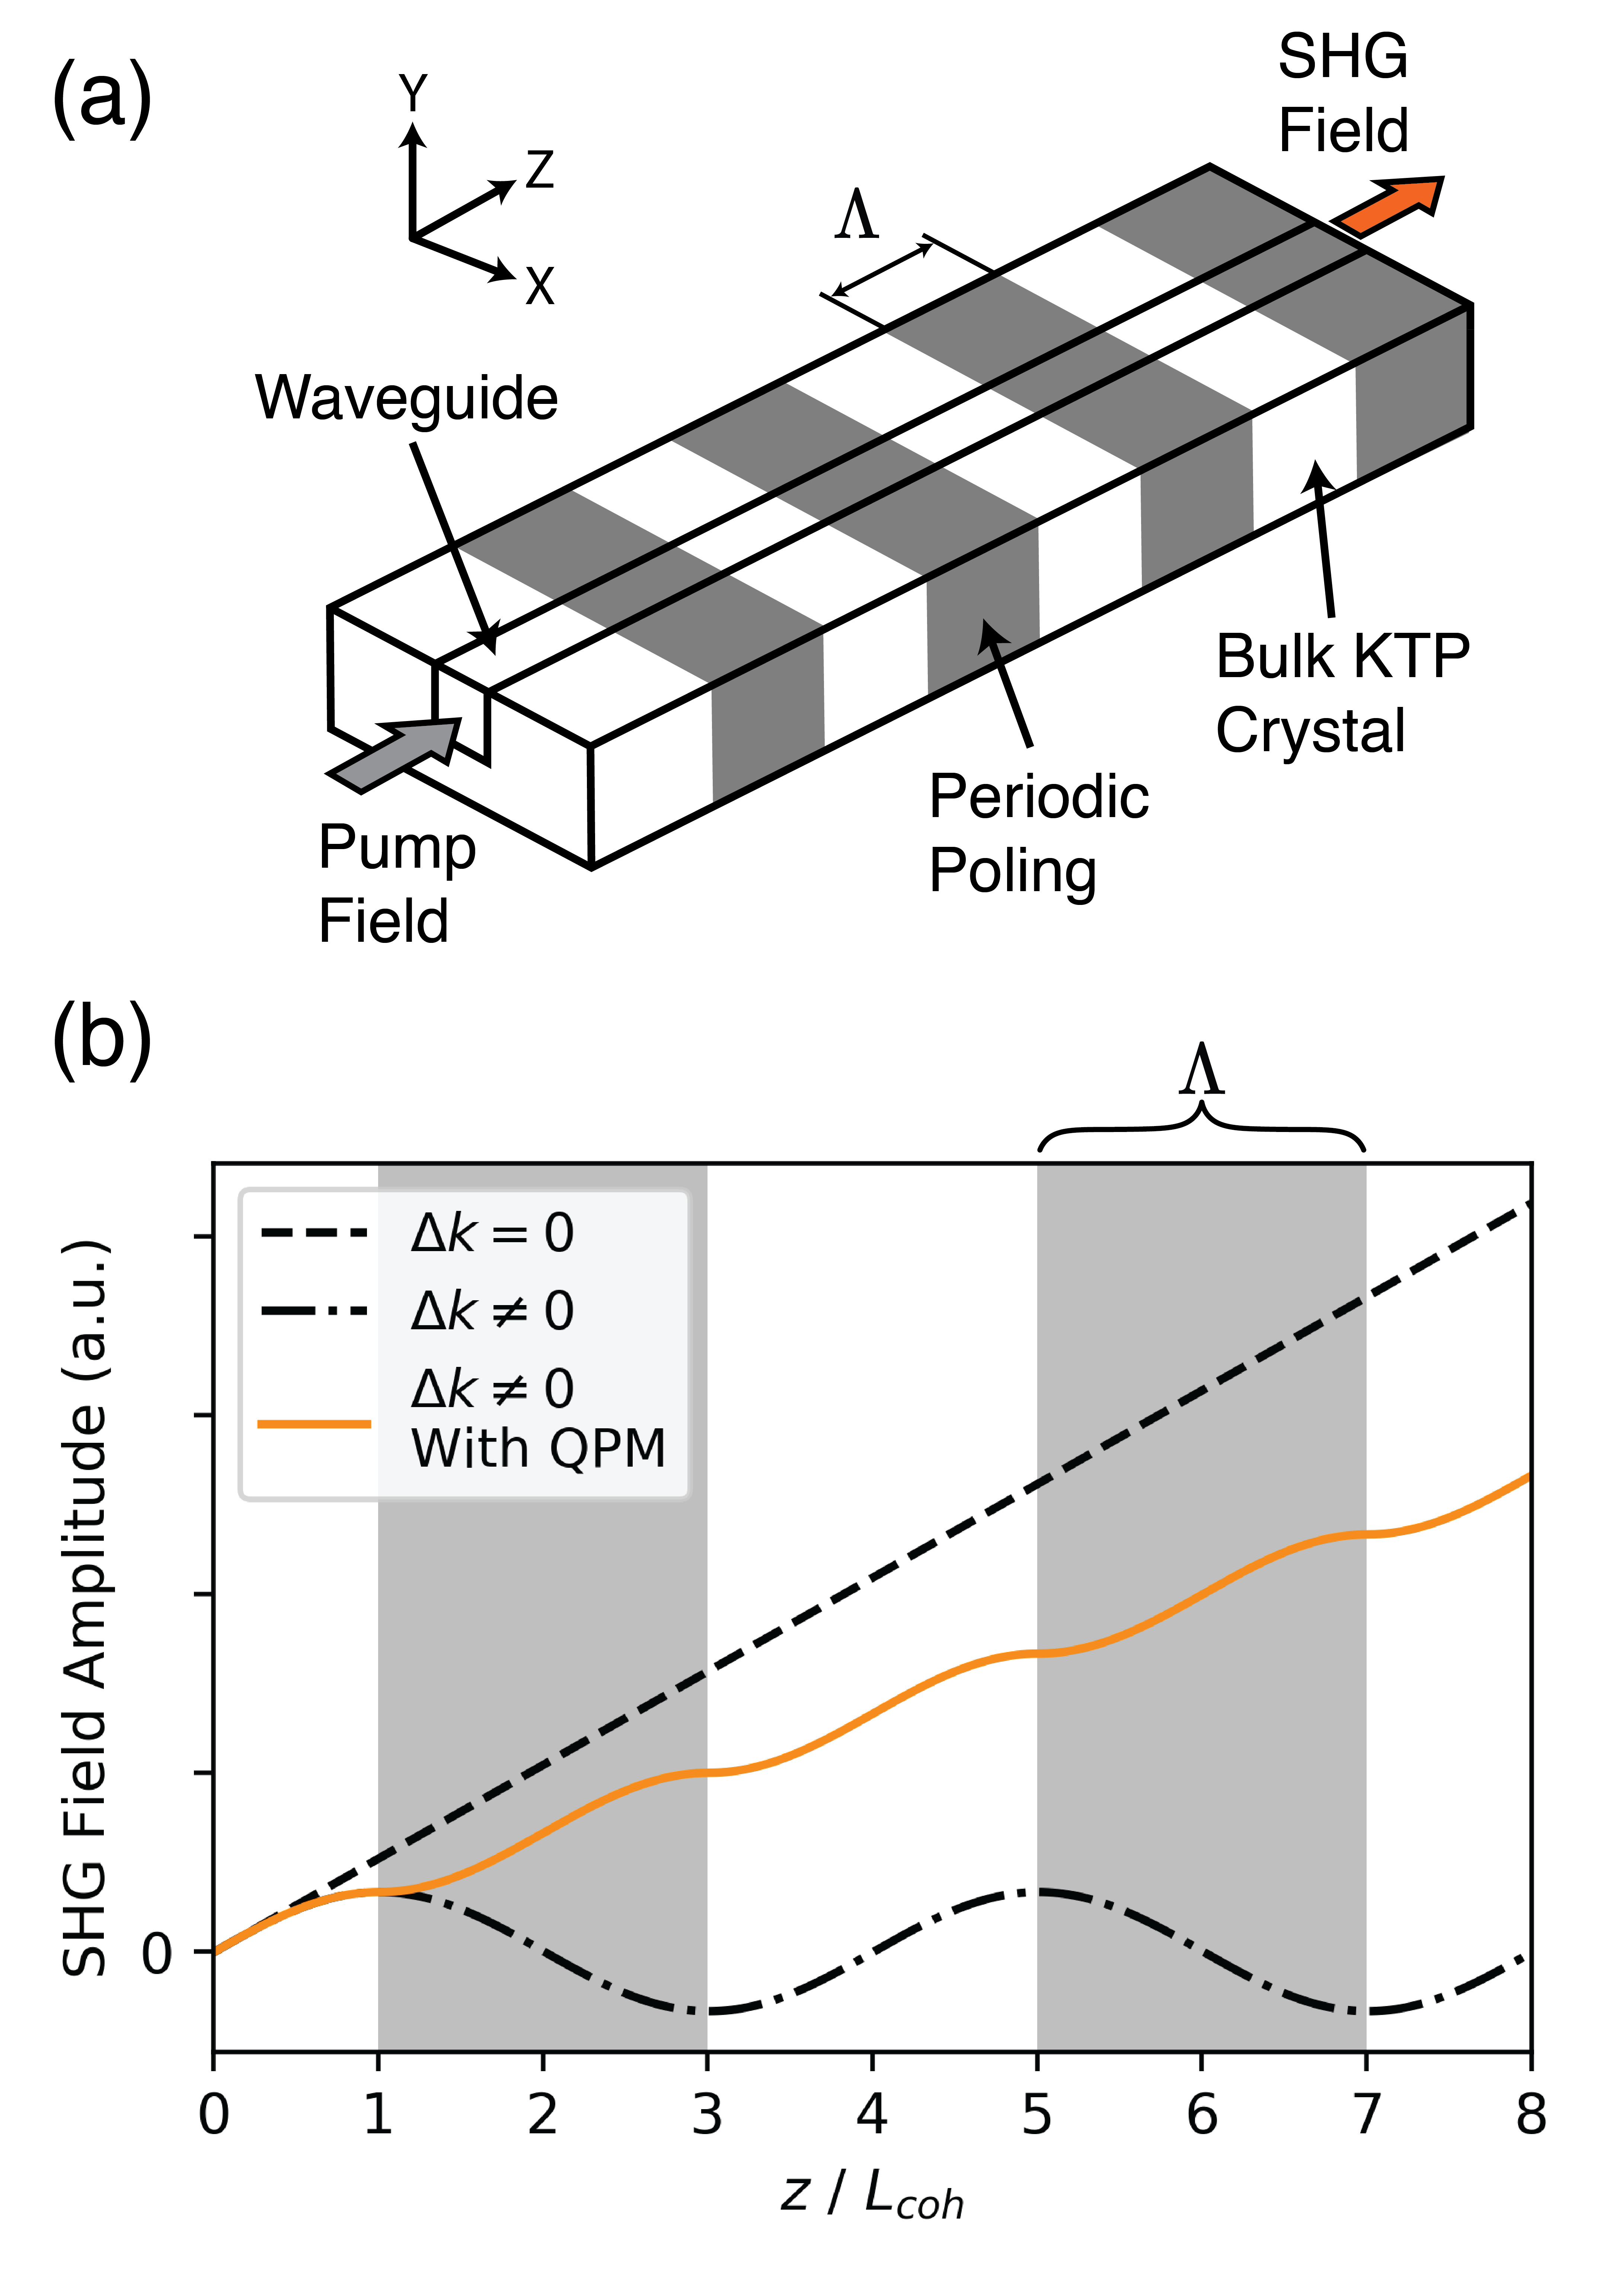
\includegraphics[width = 0.36\textwidth]{pedagogy}
	\caption{(a) Diagrammatic view of SHG chip showing one waveguide with poling period period $\Lambda = 2 L_{coh}$. (b) Comparison of SHG field power under different phase matching configurations as a function of interaction length. With perfect phase matching $\Delta k = 0$, the output power rises linearly as function of length. However with $\Delta k \neq 0$ in bulk crystal the field power will oscillate. Finally, if the sign of $\chi^{(2)}$ is reversed in the grey sections to give QPM, the resulting SHG field amplitude will increase monotonically with length, with only a slight reduction in amplitude compared to perfect phase matching.}
	\label{fig:pedagog}
\end{figure}

\section*{Waveguide Simulation}

\begin{figure*}
	\centering
	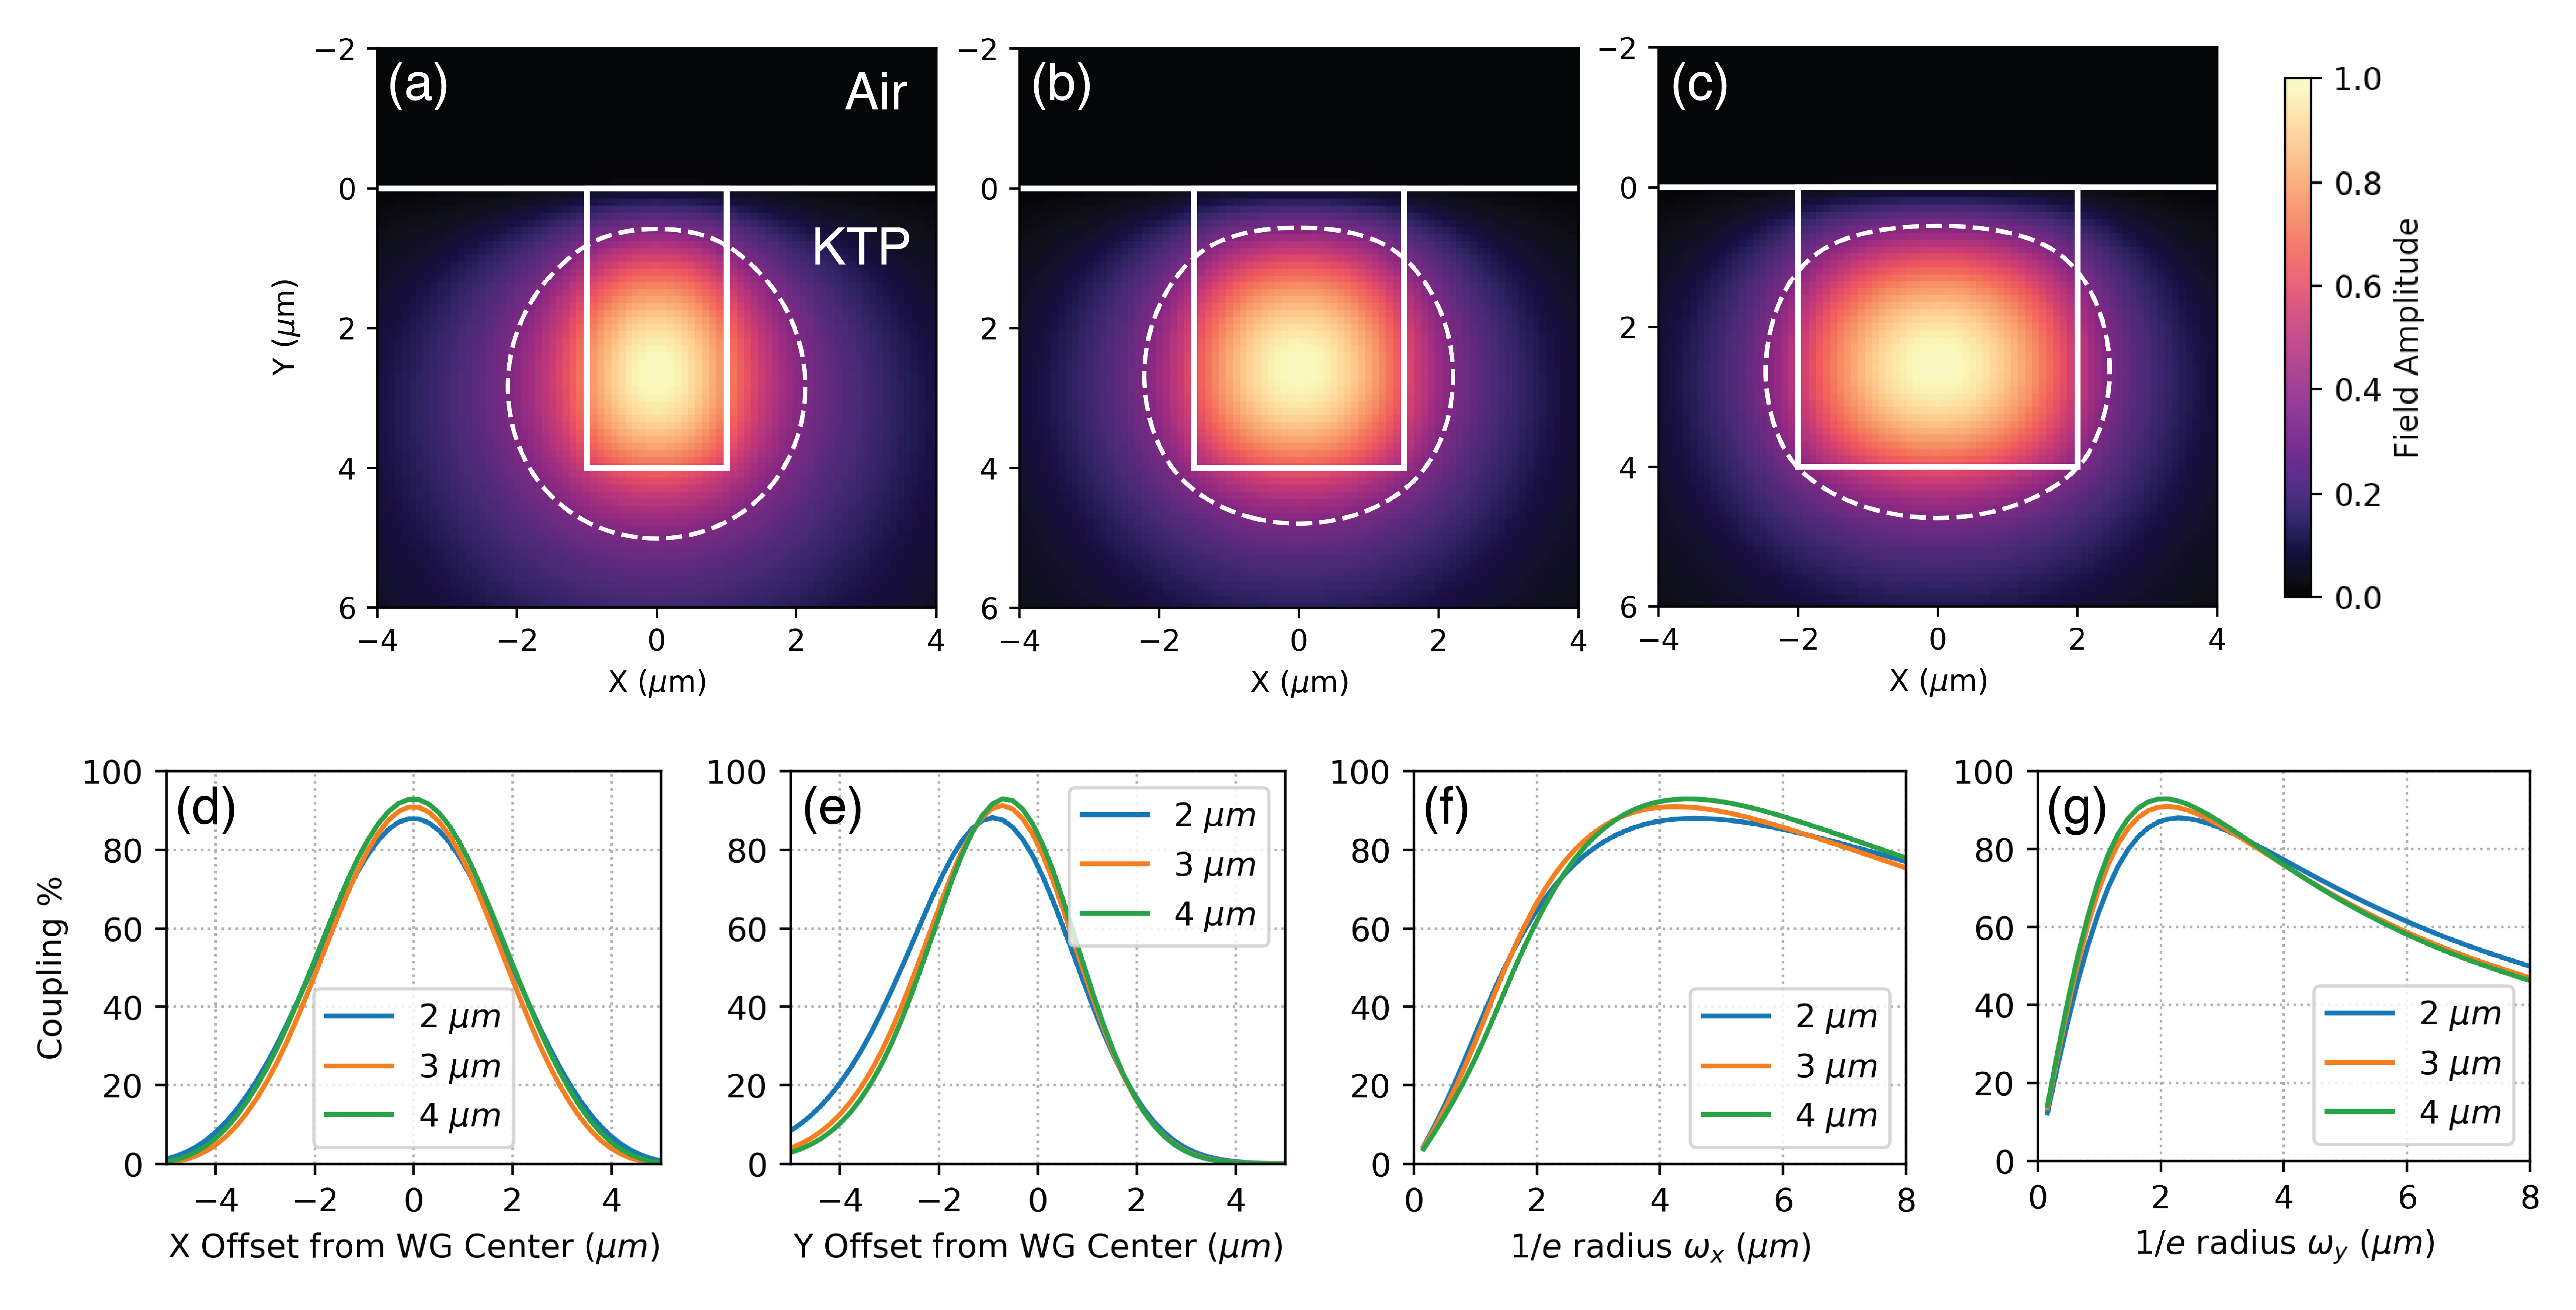
\includegraphics[width = \textwidth]{WG_sim_fig}
	\caption{Waveguide Simulations. (a), (b) and (c) show simulated modes for 2, 3 and 4 \textmu m waveguides respectively. The central white rectangle marks the boundary of the simulated waveguide, with bulk KTP $y>0$ and air $y<0$. Dashed white lines indicate the $1/e$ line of constant amplitude. (d) and (e) show the effect of translational beam misalignment in $x$ and $y$ on the coupling efficiency, assuming the optimum beam radius. (f) and (g) show the effect of beam radius in $x$ and $y$ on the coupling efficiency. Optimal translational alignment is assumed, are the non-varied axis is also assumed to be optimal.}
	\label{fig:wgsim}
\end{figure*}	

The crystal used (AdvR Inc.) is a 1.2 cm periodically-poled potassium titanyl phosphate (KTP) chip with 30 embedded waveguides, and a poling period of $\sim$ 11.52 \textmu m. The waveguides are 2, 3 and 4 \textmu m in width, with an approximate height of 4 \textmu m. Having many waveguides allows for tolerance of manufacturing inconsistencies and increases the probability of a suitable waveguide for the specific wavelength desired. The waveguides are created in bulk KTP by patterning a mask on the crystal and then immersing it into a molten metallic salt that acts as an ion source. Ions from the molten salt exchange with K ions in the KTP where the mask exposes the crystal. This results in a slight index change in the waveguide ($\sim 1.84$) compared to the bulk KTP ($\sim 1.83$). The ion diffusion rate is dependant on the crystal axes and the crystal is cut so that the diffusion rate into the crystal perpendicular to the surface is much faster than parallel to the surface. This produces a sharp index change on the sides of the waveguide, but a graded index change on the bottom of the waveguide.

Using the waveguide design software OptiBPM, all three waveguide dimensions were simulated to determine the waveguide modes, which are shown in Fig. \ref{fig:wgsim} (a), (b), and (c). The exact profile of the graded index along the bottom the waveguide is not known, therefore all waveguide boundaries are assumed to be sharp. This assumption still allows for an accurate $x$ mode width, and places a lower bound on the $y$ mode height. 

\section*{Laser Characterization}

\begin{figure}
	\centering
	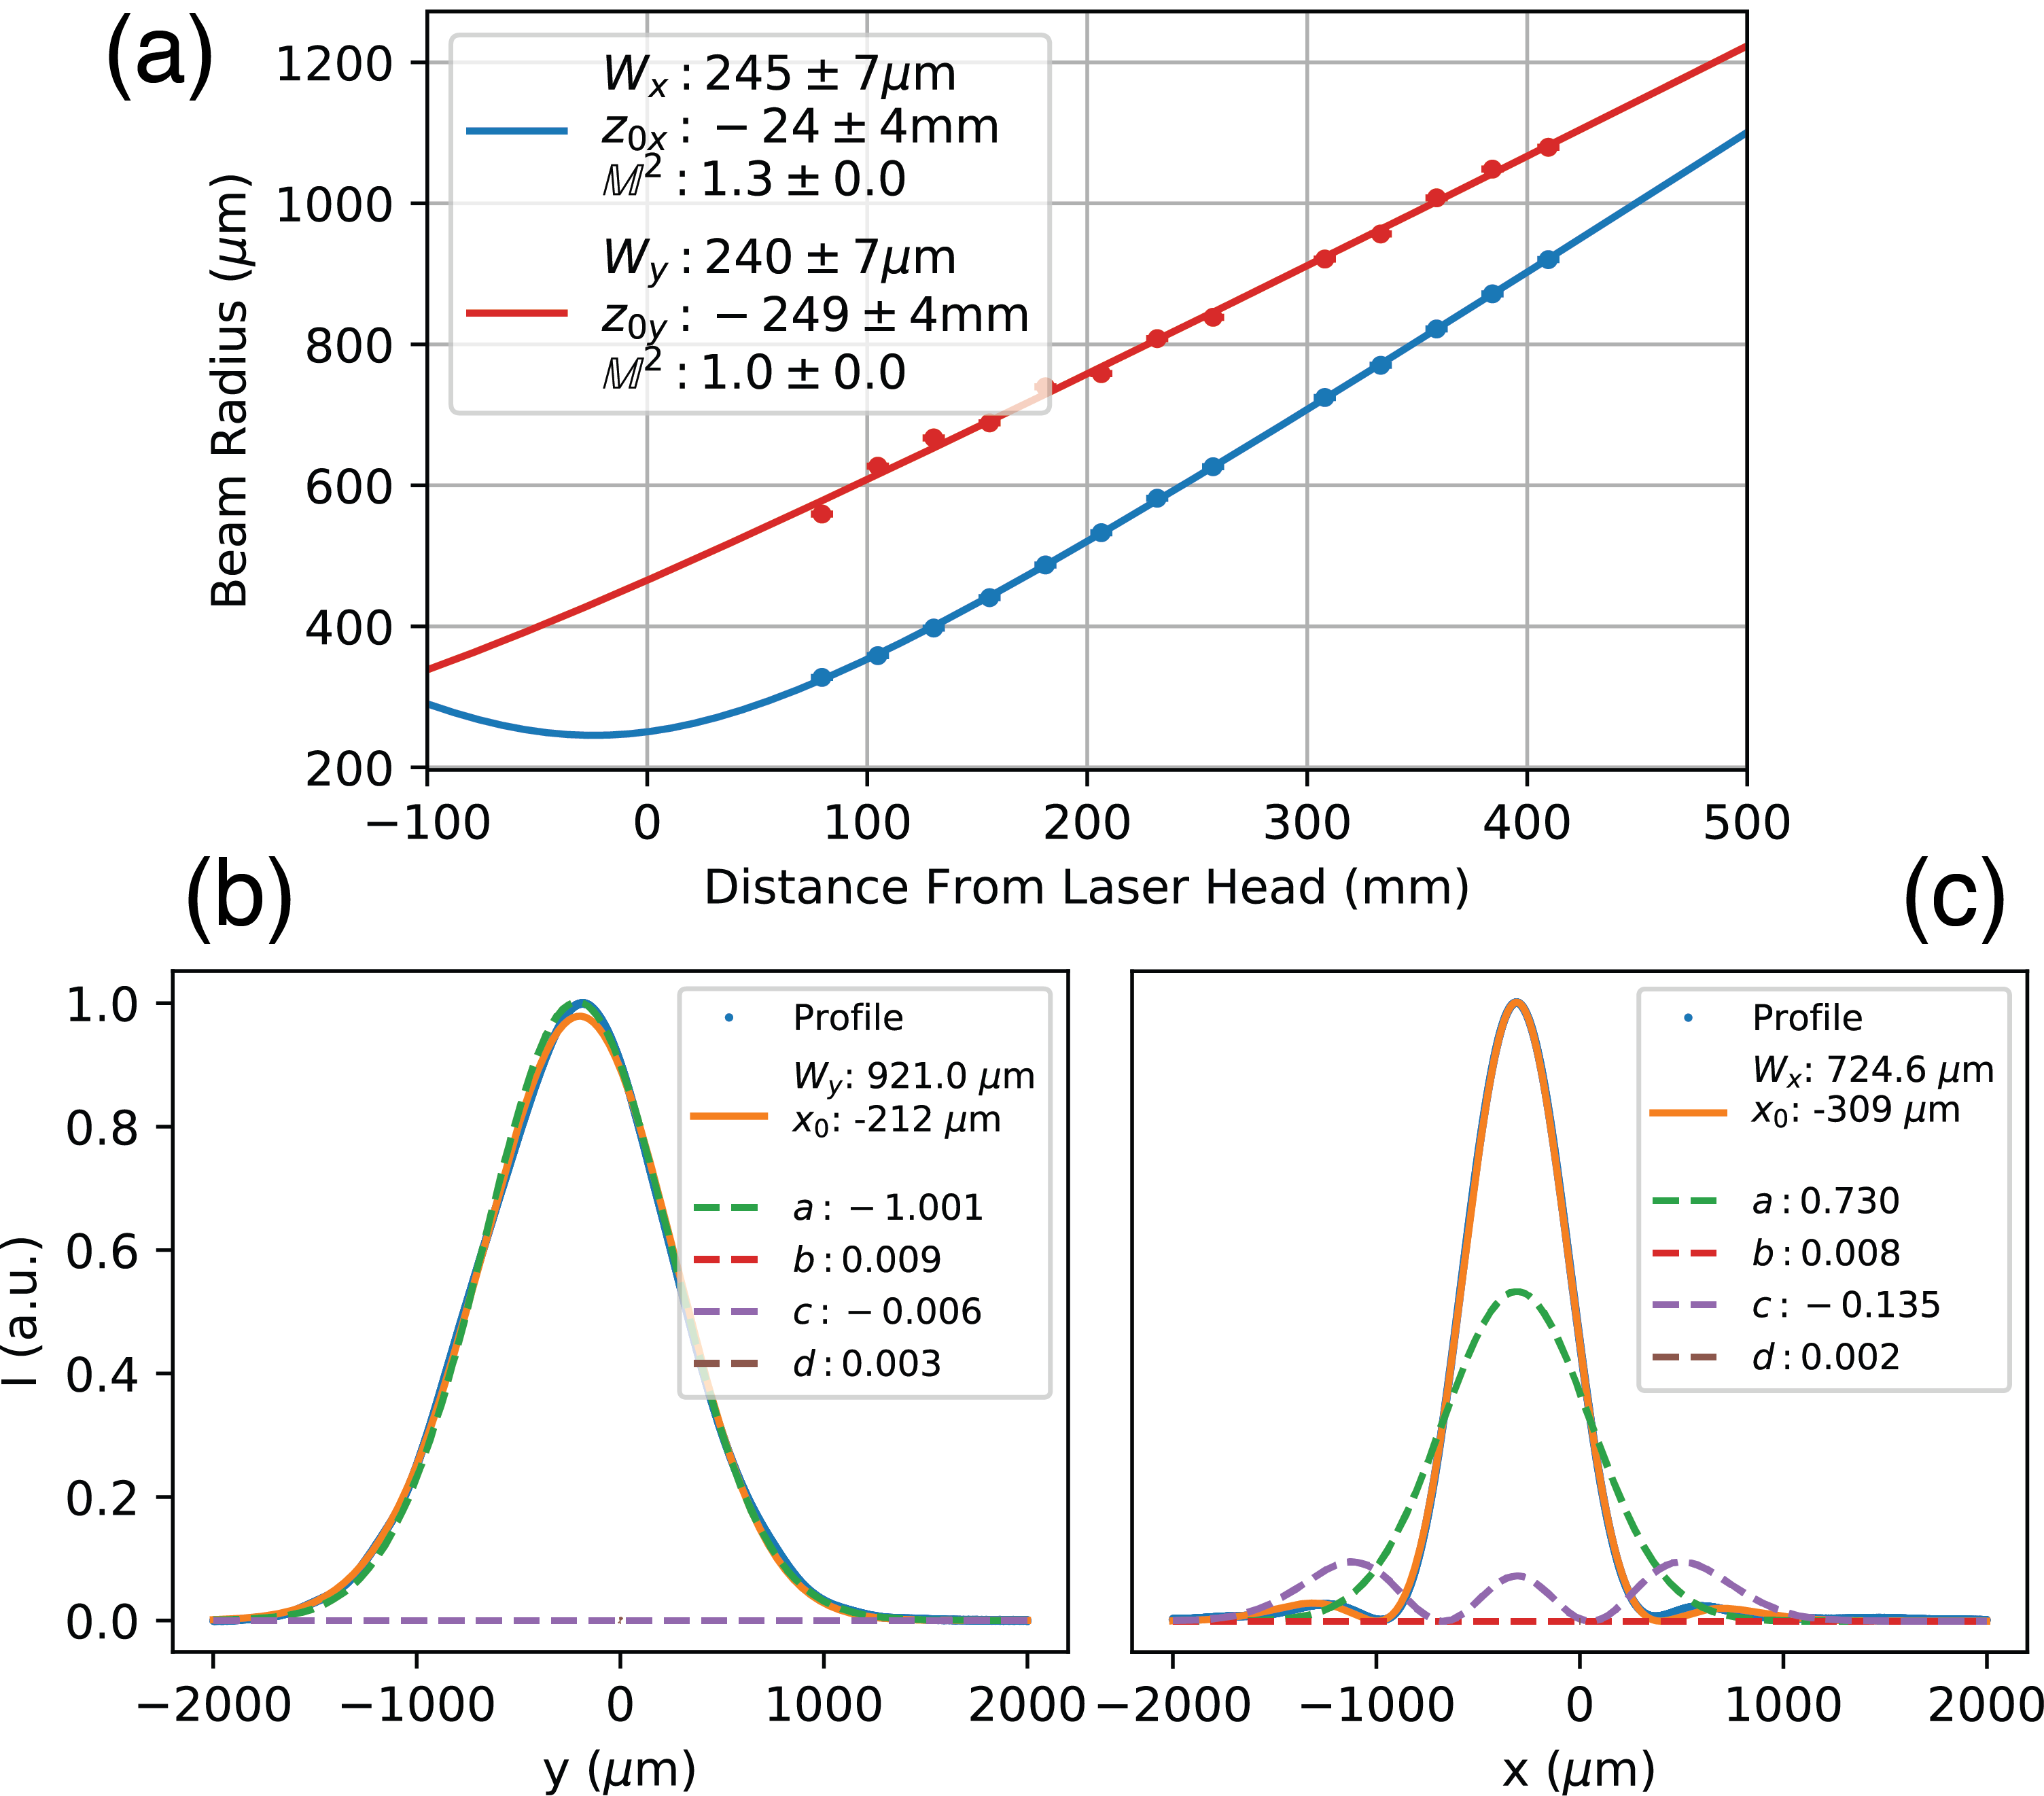
\includegraphics[width=0.49\textwidth]{propag_fig}
	\caption{Laser Characterization. (a) shows the fit of the Gaussian propagation equation \ref{equ:GP} to the $x$ (blue) and $y$ (red) axes of the pump laser beam. $W_x$, $W_y$ and $z_{0x}$, $z_{0y}$ are the $1/e^2$ waist radii and waist locations of the $x$ and $y$ components respectively. Error in beam radius is derived from the profile fits and error in distance measurement is estimated. (b) and (c) show fits of Equation \ref{equ:HG} to to the $x$ and $y$ components of the beam at 333 mm from the laser head, as a representative beam profile fit. The individual Hermite-Gaussian components are plotted in addition to the overall fit, with their respective coefficient values being given.}
	\label{fig:laserchar}
\end{figure}

To design the optical system and precisely control the pump field profile at the waveguide input, the beam produced by the pump laser must be well understood. The pump laser is an external cavity tuneable diode laser (ECDL) (Toptica Photonics DLPro). With a tiltable diffraction grating this design allows for coarse tuning of the wavelength over $\sim$80 nm, and mode hop free fine tuning using piezo control over 20GHz ($\sim$ 0.1 nm).

The laser diode silicon has a high aspect ratio, which produces a highly elliptical Gaussian beam. The laser head contains cylindrical beam-shaping optics to reduce the ellipticity, however the laser diode was rotated relative to the axes of the cylindrical lenses. As a result, different segments of the elliptical Gaussian beam were being focused differently along the optical path, producing a "rotating ellipse" effect in the beam. In order to correct the diode misalignment, the laser diode was carefully rotated to be in line with the cylindrical lens axis. Correct diode alignment also allows for correct alignment of optics further along the optical path.

The beam is then profiled at several points along the optical axis with a scanning slit beam profiler (ThorLabs BP104-IR), which generates an intensity profile along the $x$ and $y$ axis of the beam. The coordinate system of the beam is the same as the coordinate system of the waveguide shown in Fig. \ref{fig:pedagog} (a). The resulting intensity profiles are fit with a single dimension Hermite-Gaussian intensity profile
\begin{equation} \label{equ:HG}
	I(S) = \mathbb{G}^2_{0,1,2,3} \left[ \frac{\sqrt{2} (S - S_0)}{W_{S}} \right],
\end{equation}
where S is $x$ or $y$, and
\begin{equation*}
\mathbb{G}_{0,1,2,3}(u) = e^{\left( -u^2 / 2 \right)} (a \cdot \mathbb{H}_0(u) + b \cdot \mathbb{H}_1(u) + c \cdot\mathbb{H}_2(u) + d \cdot\mathbb{H}_3(u)).
\end{equation*}
$\mathbb{H}_n(u)$ is the Hermite polynomial of order $n$ and $a,b,c$ and $d$ are the coefficients for each order. Each intensity profile is first fit with a Gaussian to determine $x_0$ or $y_0$, which varies depending on the position of the profiler at the time of the measurement. This parameter is subsequently fixed for all further fitting. The mode composition of the beam remains constant as it propagates, and therefore all of the profiles for one axis are fit simultaneously with equation \ref{equ:HG}, with the requirement that $a,b,c, \text{and } d$ are equal for all profiles in that axis. Each profile is fit with an independent radius $W_{S}$. These radii are then fit with the Gaussian propagation equation
\begin{equation} \label{equ:GP}
	W(z) = W_0 \cdot \sqrt{1 + \frac{\mathbb{M}^2 (z - z_0)}{Z_r}},
\end{equation}
where $W_0$ is the waist radius, $z_0$ is the waist location, and $Z_r$ is the Rayleigh range. $\mathbb{M}^2$ is a measurement of the beam quality, with $\mathbb{M}^2=1$ indicating a perfect Gaussian beam, and $\mathbb{M}^2>1$ indicating a greater divergence angle for the same waist size. An $\mathbb{M}^2$ of 1.3 is consistent for a quality diode laser.
The Hermite-Gaussian fits shown in Fig. \ref{fig:laserchar} (b) and (c) indicate that the $x$ axis of the beam has a non-negligible second order (coefficient $b$) component, while the $y$ component is almost entirely zero order. This is also confirmed in the Gaussian propagation fit shown in Fig. \ref{fig:laserchar} (a), with an $\mathbb{M}^2>1$, as the second order component increases the effective size of the beam in the $x$ axis. 

\section*{Maximising Coupling}

\begin{table}
	\centering
	\begin{tabular}{@{}cllllll@{}}
		\toprule
		WG (\textmu m) & $W_X$, $W_Y$ (\textmu m) & $\nu$ & $\kappa$ & $\beta$ & $\eta$ & $P_{SHG}$ (mW)\\
		\midrule
		2 & 4.57, 2.30 & 91 \% & 88 \% & 73 \% & 81 \% & 4.59 \\
		3 & 4.24, 2.10 & 91 \% & 91 \% & 73 \% & 79 \% & 4.79 \\
		4 & 4.46, 2.04 & 91 \% & 93 \% & 73 \% & 84 \% & 5.31 \\
		\bottomrule
	\end{tabular}
	\caption{Theoretical calculations of optimum parameters for different waveguide sizes. $W_x$ and $W_y$ are the optimal pump beam beam radii, with the assumptions of waveguide index grading and measured pump beam mode content. $\nu$ is the transmission coefficient at the crystal input interface. $\kappa$ is the maximum coupling efficiency with the theoretical optimal beam radii and positions. $\beta$ is the output coupling losses at the crystal output interface and in the IR shortpass filter. $\eta$ is the conversion efficiency, measured by the manufacturer for a specific waveguide of the same size. $\eta$ may vary between waveguides of the same size. The power is calculated with equation \ref{equ:power}, using the $\nu$, $\kappa$, $\beta$ and $\eta$ values given and a pump power of 110 mW reaching the crystal.}
	\label{tabl:wgsize}
\end{table}

With an understanding of the waveguide and pump modes, the coupling efficiency $\kappa$ between the waveguide and pump beam is calculated with the overlap integral
$$
	\kappa = \frac{\left[ \int A B^\ast_m ds\right]^2}{\int A A^* ds \int B_m B^\ast_m ds}
$$
where $A$ is the pump electric field amplitude and $B_m$ is the waveguide mode. The spacial extent, wavefront curvature and mode orders must be matched as closely as possible to maximize the coupling. To determine the maximum possible coupling and also establish intuition for which parameters are most important, the coupling efficiency is calculated as a function of beam offset and radius. These results are presented in \ref{fig:wgsim} (d)-(g) for all three waveguide dimensions. All waveguide dimensions have very similar dependance on offset and radius, with the 2 \textmu m waveguide deviating the most. While the offset dependance is roughly Gaussian in shape and similar in $x$ and $y$, the radius dependance more complicated, and different in the beam axes. In both axes, larger beam radii reduce the coupling efficiency less than smaller beam radii. The beam dimensions with the best coupling are presented in Table \ref{tabl:wgsize}. 

The theoretical maximum coupling is calculated with the optimal beam dimensions and positions for each waveguide. In the coupling calculations, the pump beam is a Hermite-Gaussian intensity profile using the measured Hermite-Gaussian coefficients of the pump laser. Therefore, the optimal beam radius in the $x$ axis is significantly larger than the $y$ axis in order to fill the waveguide with the central mode. The pump beam is assumed to be focused on the waveguide face and therefore at the waist of a Gaussian beam with flat wavefronts, giving constant phase for the whole beam area. There is no anti-reflective coating on the waveguides, and the chip face is polished at an $\sim 8 \degree$ angle to minimize backreflections. The chip is therefore placed at a 6.8$\degree$  angle relative to the beam axis to refract the beam into the chip parallel to the waveguides. This results in a 9.4 \% loss due to reflection for the s-polarized beam, which is taken into account in the input transmission coefficient $\nu$. Similarly, the crystal output interface losses are also 9.4 \%, with an addition loss of 20 \% at the shortpass filter. These losses are taken into account in the ouput transmission coefficient $\beta$.

The power produced in the non-depleted pump approximation (integrating equation \ref{equ:a2dz}) is given by
\begin{equation} \label{equ:power}
	P_{SHG} = \beta \eta \cdot (\nu \kappa \cdot P_{pump})^2,
\end{equation}
where $\eta$ is the conversion efficiency. $\eta$ was measured when the chip was produced for three specific waveguides, one of each size, assuming that 100\% of the generated SHG light is collected. $\eta$ is not necessarily dependant on waveguide size but is dependant on $\chi^{(2)}$ and the waveguide length, with many other particular experimental factors for each individual waveguide. The conversion efficiency $\eta$ is only fully valid for the specific waveguide for which it has been measured, but does allow for an approximate calculation of the maximum possible power given in Table \ref{tabl:wgsize}. These calculations indicate that the 4 \textmu m waveguide will have the best coupling and produce the most power. However, the 3 \textmu m waveguides were found to have consistently higher output power, with the 2 \textmu m waveguides having the least.

\section*{Optical System}

\begin{figure}
	\centering
	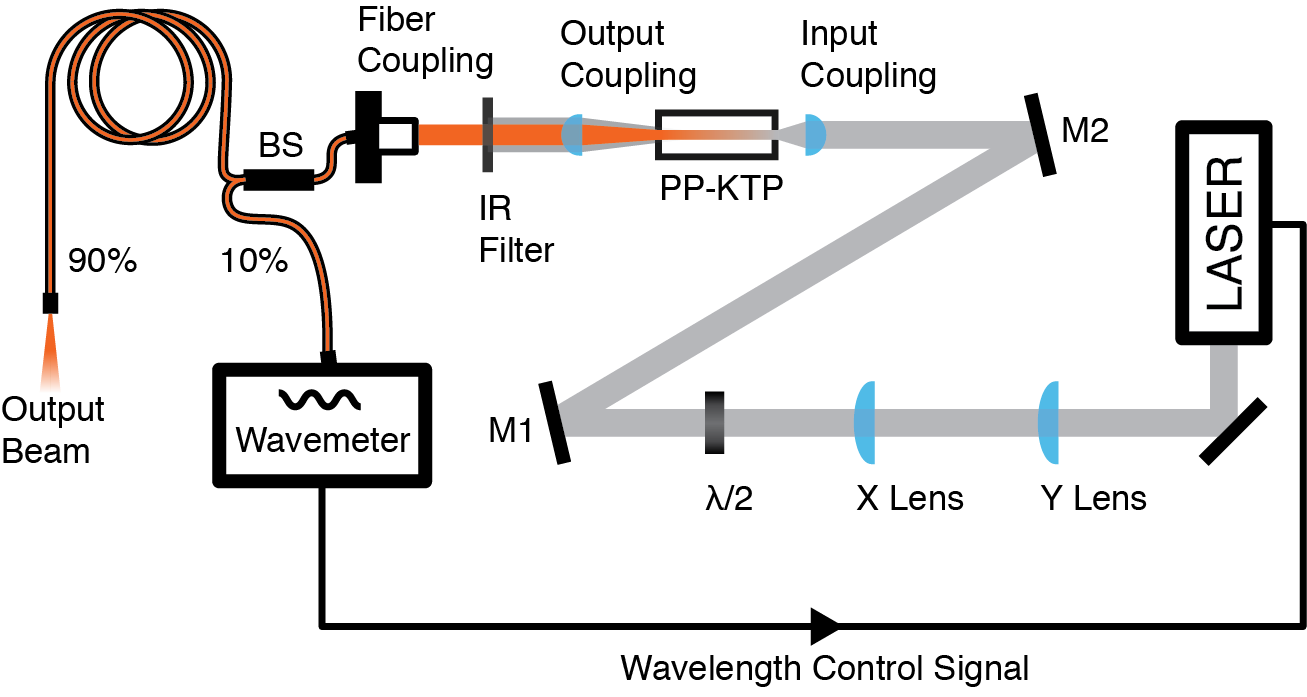
\includegraphics[width=0.5\textwidth]{diagram_presentation}
	\caption{Diagram of the optical system. LASER: $\sim$1205 nm ECDL pump. $x$ lens \& $y$ lens: Cylindrical lenses for the $x$ and $y$ axes, both mounted on cage system for adjustment. $\lambda /2$: Half wave plate in rotational mount to polarize the beam along the $y$ axis. M1 \& M2: Tip-tilt mirrors forming an additional beam walk stage. Input Coupling: Fixed $f=3.3$ mm aspheric  lens. PP-KTP: SHG chip, mounted to an x-y-z translation stage and Peltier element. Output Coupling: $f=11$ mm aspheric lens mounted on z translation stage. IR Filter: 850 nm shortpass filter to block excess IR exiting WG. Fiber Coupling: unit with a 10x objective on a z translation stage and an x-y translatable PC fiber connector. BS: Fiber 90/10 beam splitter. Wavemeter: wavemeter with a PID controller connected to the analog voltage piezo control of the laser}
	\label{fig:dia}
\end{figure}

The goal of the optical system shown in Fig \ref{fig:dia} is to shape the pump beam, couple it into the crystal waveguides and then to collect and fiber-couple the resulting light. 

\subsubsection*{Input Coupling}
The input coupling system consists of four sections. The first is two cylindrical lenses, one in each beam axis, that roughly collimate the beam and determine the radius. These can be moved freely along a cage system in order to fine tune the beam size and find the maximum coupling. A half wave plate is used to  rotate the polarization of the beam in line with the $y$ axis. Then mirrors M1 and M2 form a beam walk system that allows for precise adjustment of the angle and position of the beam entering into the final component, the input coupling lens. An aspheric lens was chosen to minimize spherical aberrations and keep the beam wavefronts as flat at the focus as possible. However, this aspheric lens has a design wavelength of 860 nm, significantly different from 1205nm wavelength it is being used to focus. The final spot size is also not diffraction limited and the input beam to the lens is not perfectly collimated. Due to these factors it is uncertain if the lens is performing as expected, which would contribute to a different coupling constant than calculated.

The SHG chip is mounted to a sub-micron precision x-y-z translation stage (Luminos Cor-Align) to align the waveguides with the focused beam coming from the input coupling lens, which is fixed. The chip itself is mounted to a copper plate with thermal paste, and the copper is connected to the mounting arm with a Peltier element that can be used to control its temperature. A thermocouple mounted in the copper allows for PID control of the chip temperature, changing its optimal SHG frequency by affecting the index of refraction and the thermal expansion of the periodic poling. 

	
\subsubsection*{Output coupling}
The output coupling and control system also consists of four sections. The output coupling lens collects and collimates the output from the end of the chip waveguide. The chip produces significant stray light which either escapes from the waveguide or is generated in the bulk KTP. However we assume that any light that can be eventually coupled to a fiber will exit the waveguide with an NA of $\sim$0.2. A shortpass filter removes the remaining IR pump beam to keep the output single wavelength. Fiber-coupling the 602nm output allows it to be easily routed and used for different applications. It also has the additional advantage of being easily and efficiently split using a fiber beamsplitter. A portion of the output is redirected to a wavemeter that precisely measures the output wavelength. As the generated wavelength is precisely half the input wavelength, an error signal from the measured crystal output wavelength is fed to a PID controller to create a control signal for the laser piezo voltage. This feedback loop controls the pump laser's wavelength with fm precision. 
		
\section*{Conclusion}
The power of SHG when using a chip with integrated waveguides and periodic poling is essentially dependant on the coupling between the pump beam and the waveguides. We have been able to achieve  856 \textmu W of output power from the chip using a 3 \textmu m waveguide, with 335 \textmu W of fiber coupled output power. 856 \textmu W is only 18 \% of the maximum theoretical output power of 4.79 mW. The discrepancy in output power comes from the assumptions made in calculating the maximum power, and the difficulty of optimizing the many coupled parameters of the optical system. 

The maximum power calculation relies on the accuracy of the waveguide simulations, where we have assumed a hard index change at the bottom of the waveguide, rather than a more realistic graded index profile. This assumption was made because the graded index is not accurately known, and results in a smaller optimal $W_y$ than reality. The maximum power is also dependant on $\eta$, however the specific waveguide we are using is the waveguide for which the 3 \textmu m $\eta$ was measured by the chip manufacturer AdvR, therefore this value is accurate. Additionally, the aspheric input coupling lens is being used at a wavelength significantly different than its design wavelength, which may be affecting both the actual spot size on the crystal, and the wavefront curvature at the waveguide face. In the calculated coupling factor the pump beam is assumed to have constant phase over its whole area. The theoretical coupling factor assumes perfect alignment and spot size control, and should be treated as an upper bound of the coupling possible. Finally, the squared dependance on the coupling factor results in significant power differences for small coupling factor differences. An output power of 856 \textmu W corresponds to a coupling efficiency $\kappa$ of 38 \%, a less significant discrepancy from the maximum $\kappa$ of 91 \% than the discrepancy in output power.

The optical system has 18 degrees of freedom, almost all of which are interdependent or correlated, resulting in a system that is difficult to optimize and has many local maxima. Reaching optimal alignment (and therefore maximum output power) can generally be achieved by finding the local maximum for each parameter, and then iterating through the remaining parameters. However, this is not the case for the position of the $x$ and $y$ cylindrical lenses that determine the beam size on the waveguide face. Moving these lenses shifts the beam position more than it affects the beam profile, and ideally these lenses should be initially fixed in the best position while the rest of the system is optimized around them. Fixing the lenses requires that the simulations and calculations previously discussed be perfectly accurate. 

Finally, the fiber-coupling losses, equivalent to a 39 \% coupling efficiency, are likely due to significant higher order mode content being generated in the waveguide as well as stray, unguided light. Higher order modes contribute to the power measurement after the crystal, but cannot be coupled into a single mode fiber, reducing the fiber-coupled power measurement. 

The next steps for this project are to further improve the coupling through better lens placement, and to increase the wavelength tuning range. The dependance of the optimum wavelength on temperature must be better understood in order to consistently tune the crystal for a particular output wavelength. 

\section*{Acknowledgements}
Rigel Zifkin for his previous work on the project and everyone in the Childress lab for their knowledge and help. 

	
\pnasbreak
\section*{References}

% \pnasbreak splits and balances the columns before the references.
% Uncomment \pnasbreak to view the references in the PNAS-style
% If you see unexpected formatting errors, try commenting out \pnasbreak
% as it can run into problems with floats and footnotes on the final page.
%\pnasbreak

\bibliography{references}

\end{document}